\chapter{Develop new analyses with Harmony}

This part explains step-by-step how to add the Harmony plugin in your Eclipse development environment, launch harmony inside eclipse, and how to create a new analysis.


\section{Install the Harmony plugin}
Firsts things first, you need to install Eclipse, from \url{http://www.eclipse.org/downloads/}. We recommend Eclipse Classic, as it is packaged with the Plugin Development Environment.

Once Eclipse downloaded and unzipped, run it, and install a new plugin via the menu \texttt{Help $\rightarrow$ Install new software}. In the "work with" field, type \url{http://se.labri.fr/data/harmony/update-site}. Select the \texttt{Harmony} category, and install the selected plugins (see \figurename~\ref{fig:install-harmony}).

Restart Eclipse, the harmony plugins are loaded in your Eclipse configuration.

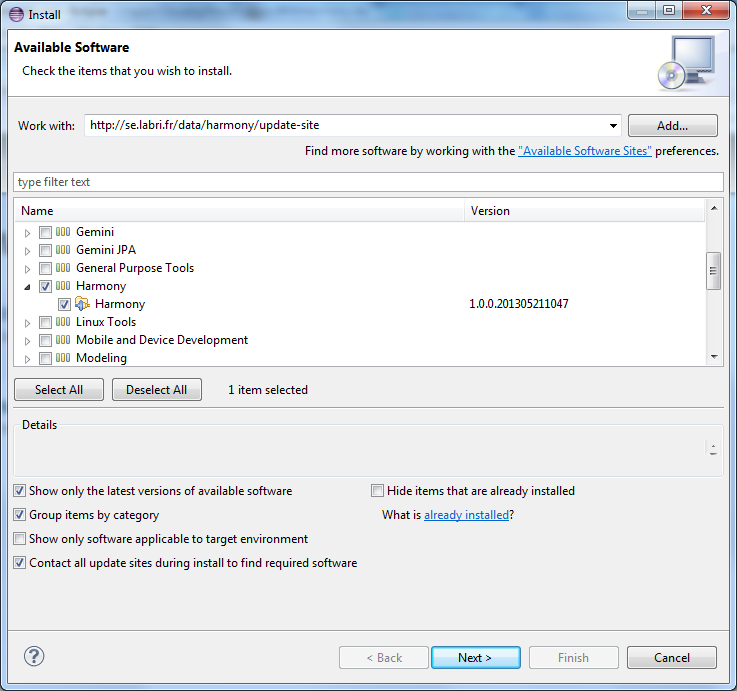
\includegraphics[width=5in]{install-harmony}

\section{Run Harmony within Eclipse}

The next step is to import the \texttt{harmony.core} plugin in your workspace.
You can do this via the \texttt{File $\rightarrow$ Import} menu.

Then select \texttt{Plugin and Fragments}

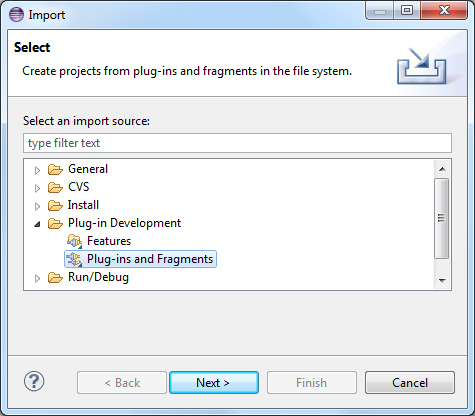
\includegraphics[width=2.5in]{import-menu}
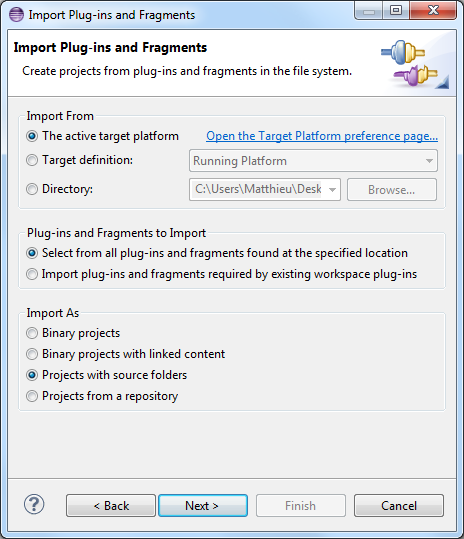
\includegraphics[width=2.5in]{import-plugin-menu}

\section{Create a new analysis}


